% This is a Basic Assignment Paper but with like Code and stuff allowed in it, there is also url, hyperlinks from contents included. 

\documentclass[11pt]{article}

% Preamble

\usepackage[margin=1in]{geometry}
\usepackage{amsfonts, amsmath, amssymb}
\usepackage{fancyhdr, float, graphicx}
\usepackage[utf8]{inputenc} % Required for inputting international characters
\usepackage[T1]{fontenc} % Output font encoding for international characters
\usepackage{fouriernc} % Use the New Century Schoolbook font
\usepackage[nottoc, notlot, notlof]{tocbibind}
\usepackage{listings}
\usepackage{xcolor}
\usepackage{blindtext}
\usepackage{hyperref}
\hypersetup{
    colorlinks=true,
    linkcolor=black,
    filecolor=magenta,      
    urlcolor=cyan,
    pdfpagemode=FullScreen,
    }

\definecolor{codegreen}{rgb}{0,0.6,0}
\definecolor{codegray}{rgb}{0.5,0.5,0.5}
\definecolor{codepurple}{rgb}{0.58,0,0.82}
\definecolor{backcolour}{rgb}{0.95,0.95,0.92}

\lstdefinestyle{mystyle}{
    backgroundcolor=\color{backcolour},   
    commentstyle=\color{codegreen},
    keywordstyle=\color{magenta},
    numberstyle=\tiny\color{codegray},
    stringstyle=\color{codepurple},
    basicstyle=\ttfamily\footnotesize,
    breakatwhitespace=false,         
    breaklines=true,                 
    captionpos=b,                    
    keepspaces=true,                 
    numbers=left,                    
    numbersep=5pt,                  
    showspaces=false,                
    showstringspaces=false,
    showtabs=false,                  
    tabsize=2
}

\lstset{style=mystyle}

% Header and Footer
\pagestyle{fancy}
\fancyhead{}
\fancyfoot{}
\fancyhead[L]{\textit{\Large{SRS for Attendance Assistant}}}
%\fancyhead[R]{\textit{something}}
\fancyfoot[C]{\thepage}
\renewcommand{\footrulewidth}{1pt}



% Other Doc Editing
% \parindent 0ex
%\renewcommand{\baselinestretch}{1.5}

\begin{document}

\begin{titlepage}
	\centering

	%---------------------------NAMES-------------------------------

	\huge\textsc{
		MIT World Peace University
	}\\

	\vspace{0.75\baselineskip} % space after Uni Name

	\LARGE{
		Software Engineering and Testing\\
		Second Year B. Tech, Semester 4
	}

	\vfill % space after Sub Name

	%--------------------------TITLE-------------------------------

	\rule{\textwidth}{1.6pt}\vspace*{-\baselineskip}\vspace*{2pt}
	\rule{\textwidth}{0.6pt}
	\vspace{0.75\baselineskip} % Whitespace above the title



	\huge{\textsc{
			Software Requirement Specification - \textbf{SRS} for
			\textit{"Attendance Assistant"}
		}} \\



	\vspace{0.5\baselineskip} % Whitespace below the title
	\rule{\textwidth}{0.6pt}\vspace*{-\baselineskip}\vspace*{2.8pt}
	\rule{\textwidth}{1.6pt}

	\vspace{1\baselineskip} % Whitespace after the title block

	%--------------------------SUBTITLE --------------------------	

	\LARGE\textsc{
		Assignment 1
	} % Subtitle or further description
	\vfill

	%--------------------------AUTHOR-------------------------------

	Prepared By
	\vspace{0.5\baselineskip} % Whitespace before the editors

	\Large{
		Krishnaraj Thadesar \\
		Cyber Security and Forensics\\
		Batch A1, PA 20
	}


	\vspace{0.5\baselineskip} % Whitespace below the editor list
	\today

\end{titlepage}


\tableofcontents
\thispagestyle{empty}
\clearpage

\setcounter{page}{1}

\section{Purpose}
The Aim of SRS is to specify the software product in details. In other words, it contains all necessary and important information that the product team should be aware of in order to create the software. This document explains this with respect to the \textbf{Application Software} in Question - \textit{Attendance Assistant}. The Purpose is to solve the below mentioned Problem statement. The Proposed solution is to create an App, that would run on Android and iOS, to facially recognize the faces of students, thereby making the process of recording their presence faster than the conventional methods.  

\section{Problem Statement}
\textit{The Purpose of an Attandence Assistant App is to help reduce the time taken for recording the attendance of a classroom in a school or college. The app will be able to record the attendance of a class in a matter of a few Seconds with minimum Energy Expended. It will record data on cloud, and be accessible to all the Teachers.}\\

\section{Requirements}

\subsection{Functional Requirements}
The Attandence Assistant must : 
\begin{enumerate}
    \item Be able to record the attendance of a class in a matter of Seconds.
    \item Must allow different Privileges for different Teachers, and Coordinators of a School or University
    \item Incorporate a Database to store the attendance of a class, that must have a backup in case of a system failure.
    \item Have a User Interface that is easy to use, and is intuitive.
    \item Be able to be used on a variety of Operating Systems, and be able to be used on a variety of devices.
    \item Be able to store the Records in a Cloud Database, as well as a Local one in case of a Poor internet Connection. 
    \item Be able to read the face of a person from a distance of 1-2 meters.
    \item Be able to communicate and Auto update the Attandence in the ERP management of the School or University.
    \item Be able to share the data through usual Messaging apps and save to local storage in an excel file. 
\end{enumerate}
\subsection{Performance Requirements}
\begin{enumerate}
    \item Verifing Face Data is a CPU intensive process. Therefore, it must be as optimized as possible. 
    \item The Faces of each student must be logged beforehand, and the processed app data can be stored on the cloud. This will reduce the redundant processing on the face data. 
    \item The App must incorporate multithreading, and use the CPU and GPU present on modern smartphones to its full potential.
\end{enumerate}

\section{Design Constraints}
The System is constrained in the following places: 
\begin{itemize}
    \item The Presence of a Smartphone.
    \item The presence of a good Camera on the Smartphone.
    \begin{itemize}
        \item Greater than 8 MP
        \item Having Some form of Stabalization, Optical or Electronic.
    \end{itemize}
    \item Having a decent CPU and GPU being present on the Smartphone. 
    \begin{itemize}
        \item Freaquency of 1.5 GHz or more.
        \item Multi Core.
    \end{itemize}
    \item Having a good internet connection, or a local database to store the data.
    \item The Operating System of the Smartphone must be Android or iOS.
\end{itemize}
\section{Proposed Idea}

Developing a Multi OS app, that can: 

\begin{enumerate}
    \item Run on Android and iOS.
    \item Facially identify the students in a class.
    \item Store the Information Locally and on Cloud. 
\end{enumerate}

\section{Validation and Testing}

\subsection{Testing}
\begin{enumerate}
    \item The App will have to be tested rigorously on a variety of devices, and operating systems.
    \item It will also have to be tested for facial recognition from various angles and distances. 
    \item It will have to be tested for a variety of faces and skin tones.
\end{enumerate}

\subsection{Validation}
\begin{enumerate}
    \item Validation of the Data will ultimately have to be done by teachers, and those taking the attendance.
    \item Further Validation can be done by the students, when they are able to see their attendance on the ERP of the School or University.
\end{enumerate}

\section{Design}
\begin{figure}[H]
    \begin{small}
        \begin{center}
            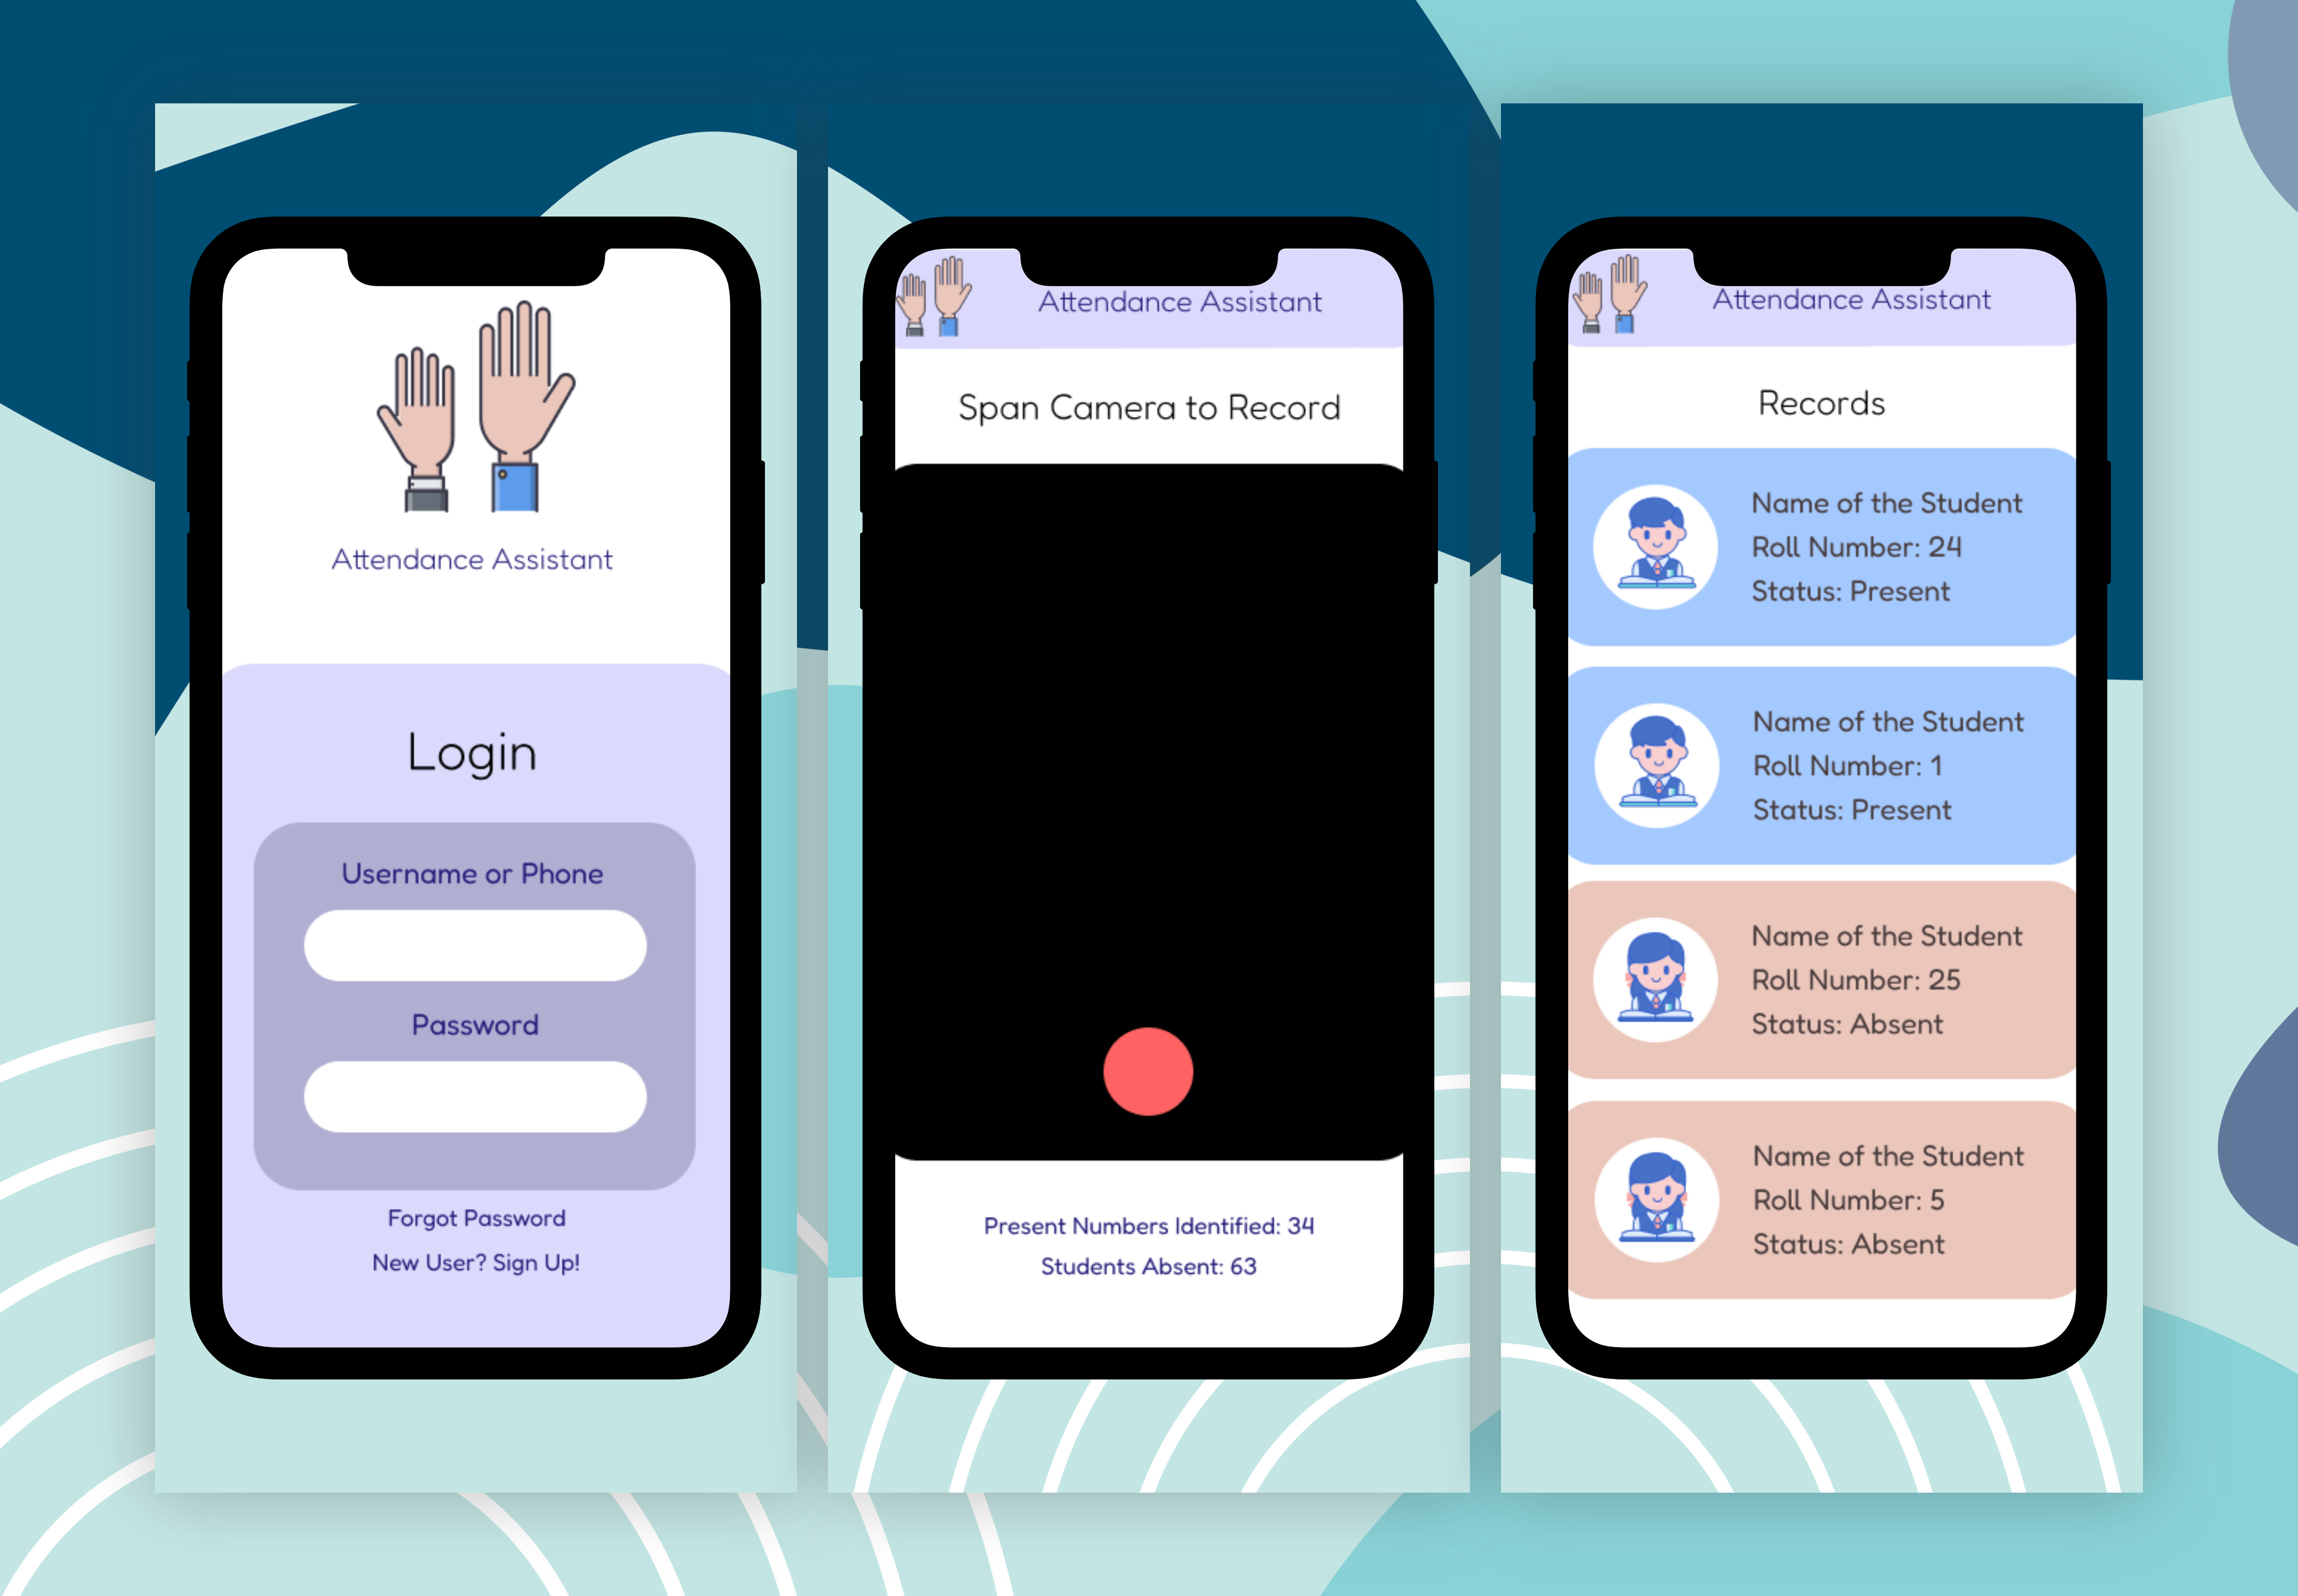
\includegraphics[scale=0.1]{app.png}
        \end{center}
        \caption{Login Page}
    \end{small}
\end{figure}

\section{Tables Generated}

\subsection{Students}

\begin{table}[H]
    \begin{tabular}{|l|l|l|l|l|}
    \hline
    Sr. No & Name of the Student & Face of the Student                               & Roll Number of the Student & PRN of the student \\ \hline
    1      & Krishnaraj Thadesar & \textless{}face\_data\_from\_opencv\textgreater{} & 20                         & 1032210888         \\ \hline
    2      & Devanshu Surana     & \textless{}face\_data\_from\_opencv\textgreater{} & 37                         & 1032201654         \\ \hline
    3      & Parth Zarekar       & \textless{}face\_data\_from\_opencv\textgreater{} & 15                         & 1032210846         \\ \hline
    4      & Rohit Jobish        & \textless{}face\_data\_from\_opencv\textgreater{} & 89                         & 1032210658         \\ \hline
    \end{tabular}
\end{table}

\section{Classes}

\begin{table}[H]
    \begin{tabular}{|l|l|l|l|l|l|l|}
    \hline
    Class ID & School & Section  & Panel \\ \hline
    1001     & SCET   & CSE      & A     \\ \hline
    1002     & SCET   & CSF      & A     \\ \hline
    1003     & SCME   & Robotics & A     \\ \hline
    \end{tabular}
    \end{table}

\section{Programs}

\begin{table}[H]
    \begin{tabular}{|l|l|l|l|}
    \hline
    P. No & School & Program Name                       & Number of  Panels \\ \hline
    1     & SCET   & Computer Science and CyberSecurity & 1                 \\ \hline
    2     & SCET   & CSE Artificial Intelligence and DS & 2                 \\ \hline
    \end{tabular}
\end{table}

\section{Professors}
\begin{table}[H]
    \begin{tabular}{|l|l|l|l|}
    \hline
    Professor ID & School & Subjets Taught & Name of Professor \\ \hline
    1001         & SCET   & CN             & Lalit Kulkarni    \\ \hline
    1002         & SCET   & {[}OS, SET{]}  & Jyoti Gavhane     \\ \hline
    \end{tabular}
    \end{table}
\section{Subjects}

\begin{table}[H]
    \begin{tabular}{|l|l|l|l|}
    \hline
    Professor ID & School & Subjets Taught & Name of Professor \\ \hline
    1001         & SCET   & CN             & Lalit Kulkarni    \\ \hline
    1002         & SCET   & {[}OS, SET{]}  & Jyoti Gavhane     \\ \hline
    \end{tabular}
    \end{table}

\section{Attendance}

\begin{table}[H]
    \begin{tabular}{|l|l|l|l|l|}
    \hline
    A.ID & Date      & Subject Name                     & PRN of Present Students                                                                                     & PRN of Absent Students      \\ \hline
    1    & 25/2/2023 & Software Engineering and Testing & \begin{tabular}[c]{@{}l@{}}{[}1032210888, \\ 1032210553,\\ 1032210937,\\ ........1032210432{]}\end{tabular} & {[}1032133234, 122312345{]} \\ \hline
    2    & 25/2/2023 & Advanced Data Structures         & \begin{tabular}[c]{@{}l@{}}{[}1032210888, \\ 1032210553,\\ 1032210937,\\ ........1032210432{]}\end{tabular} & {[}1032133234, 122312345{]} \\ \hline
    \end{tabular}
    \end{table}

\section{Delivery: Sent for Approval}



\end{document}